\section{Why does the meaning or effect of a sound change with experience and repetition?}
\label{sec:persistence}

Play an alarm call to a ground squirrel and it looks up. Play the same call again and again, and it soon goes back to feeding. That decline is biologically informative, not just a practical nuisance, because the first response and the maintained response can reflect different computations. At least four accounts produce declining curves: sensory habituation; learning that a particular caller or cue is unreliable; a shift in motivation or context that makes the sound less relevant; and temporal prediction or risk allocation. Formal criteria for habituation---stimulus specificity, spontaneous recovery, dishabituation---rule out fatigue and sensory adaptation \citep{RankinEtAl2009}, but they do not separate the other three. Similar curves do not identify a single mechanism (\figref{fig:temporal}).

\begin{figure}[tbp]
  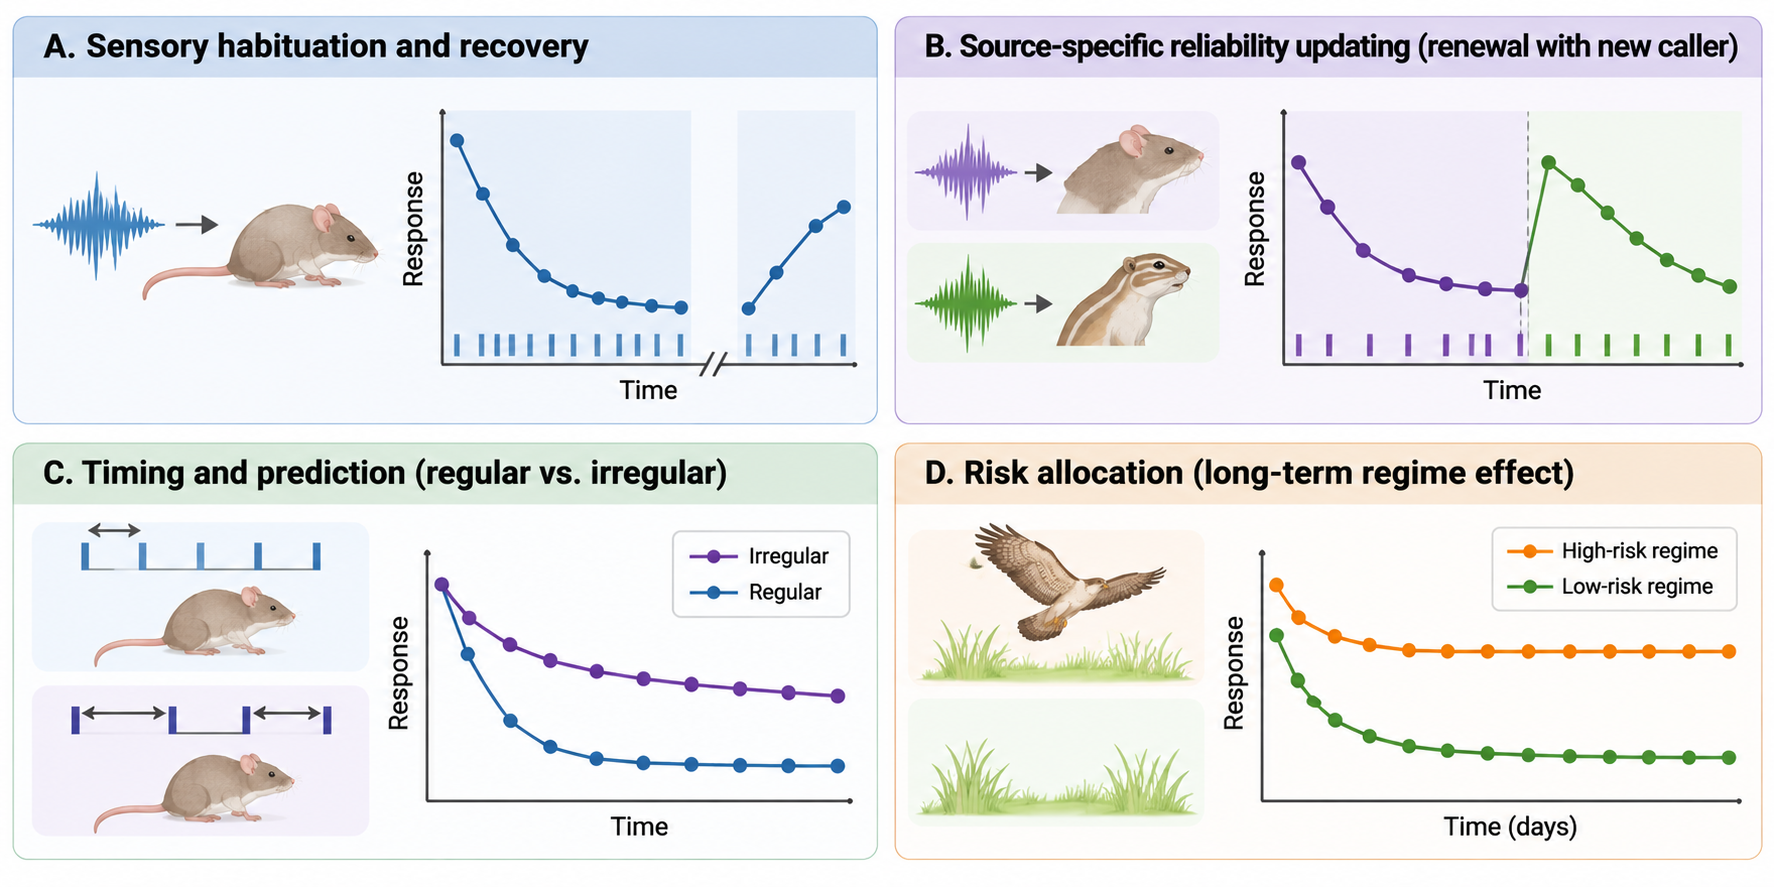
\includegraphics[width=\textwidth]{fig4_temporal_placeholder.png}
  \caption{Competing interpretations of response decline (schematic; curves idealized). (A)~Sensory habituation and recovery. (B)~Source-specific decline and renewal when the caller changes; renewal is consistent with, but does not by itself establish, reliability learning. (C)~Timing and prediction effects documented with artificial laboratory sounds. (D)~Risk allocation as a hypothesized long-term regime effect: when high-risk periods are frequent, vigilance per alarm is predicted to be lower than when they are rare. Similar curves do not identify a single process.}
  \label{fig:temporal}
\end{figure}

\subsection{Sensory habituation and recovery}
\label{sec:persistence-habituation}

Field evidence for decline specific to a caller or stimulus is strong. Richardson's ground squirrels and yellow-bellied marmots respond less across repeated calls from one individual and recover when the caller changes; in ground squirrels, a new recording from the same caller is not enough to restore responding \citep{Hare1998,BlumsteinDaniel2004}. Whether ecological significance slows habituation relative to an acoustically matched control is less clear. The main evidence is greater recovery after rest to a loud natural distress squeal than to its synthetic mimic \citep{EvansHammond1983a}. Significance does not prevent decline: rat approach to 50-kHz playback falls even when playback predicts a social encounter \citep{BerzEtAl2022}, and approach and accumbens dopamine both decline rapidly across 50-kHz presentations \citep{WilluhnEtAl2014}. Generic habituation predicts generalization across acoustically similar callers and recovery with time alone, so renewal when the caller changes already goes beyond pure sensory habituation.

\subsection{Reliability learning versus generic habituation}
\label{sec:persistence-reliability}

If receivers learn about reliability, responses should decline for a particular source and return when the caller changes or when calls are again paired with danger. Juvenile ground squirrels discount callers whose alarms are repeatedly not followed by a predator model \citep{HareAtkins2001}. Marmots do the opposite: they respond \emph{more} to experimentally unreliable callers, and they also weigh the caller's distance and the number of callers \citep{BlumsteinEtAl2004}, while familiarity alone has no detectable effect \citep{BlumsteinDaniel2004}. Discounting and closer scrutiny are both reasonable responses to unreliable information; which is favored may depend on how costly it is for the receiver to check for itself. That is a possible explanation, not a settled mechanism, and the available studies differ in species, endpoints, and paradigms. Laboratory rodents can discriminate callers \citep{VielleEtAl2021,WarrenEtAl2025}, but no laboratory study has manipulated caller reliability. Separating reliability learning from habituation requires holding the acoustic structure and the schedule as constant as possible while varying whether calls are paired with danger.

\subsection{Motivational and contextual relevance}
\label{sec:persistence-motivation}

A response can also decline because the sound has become less worth acting on, not because it is perceived differently. Approach to 50-kHz calls falls across repetitions even when the calls predict social contact \citep{BerzEtAl2022}, which suggests that motivational updating can proceed despite the call's significance. Context changes that switch mice between flight and freezing to the same sweep \citep{MongeauEtAl2003} likewise show that the action expressed tracks state. A motivational account predicts recovery when the costs of responding change---hunger, distance to refuge---without any change in the sound. Acoustic studies rarely test this.

\subsection{Temporal expectation and risk allocation}
\label{sec:persistence-timing}

When sounds arrive matters as well as what they are. At the same average interval, regularly timed startle stimuli produce more habituation than irregularly timed ones \citep{Davis1970}, and tone pulses with jittered timing prevent rapid habituation in the basolateral amygdala and can promote avoidance \citep{HerryEtAl2007}. Both studies used artificial sounds and manipulated how variable the intervals were, not the shape of their distribution. They do not show that a particular schedule would sustain responses to natural calls in the field. Accumbens dopamine recovers differently after noise depending on whether the noise was predicted \citep{GoedhoopEtAl2022}, linking expectation to a neural measure without establishing a field rule. Within natural calling bouts, call rate and structure alter vigilance \citep{BlumsteinArmitage1997,SloanEtAl2005}, yet adults may ignore rate changes in juvenile calls \citep{SloanHare2006}.
% VERIFY: SloanEtAl2005, SloanHare2006, BlumsteinArmitage1997 (not full-text checked).
Urgency within a bout is therefore distinct from the statistics of intervals over longer periods. Risk allocation predicts less vigilance per alarm when high-risk periods are frequent \citep{LimaBednekoff1999}; we found no test of this with acoustic cues in rodents.

\subsection{What competing accounts imply}
\label{sec:persistence-synthesis}

The accounts make different predictions about recovery after rest, renewal when the source changes, generalization across similar callers, dependence on whether calls have been paired with danger, and sensitivity to interval distribution when the number of events is matched. Laboratory neuroscience offers candidate mechanisms for some of these. Prefrontal and hippocampal circuits control how far learned fear generalizes to new sounds and how it is extinguished when a cue stops predicting danger \citep{ConcinaEtAl2018,QuinnEtAl2009,SierraMercadoEtAl2011}, and neuromodulatory state changes how strongly a remembered cue drives behavior (\secref{sec:mechanisms-state}). Caller-specific discounting looks like extinction restricted to one source, and renewal after a caller change looks like a failure to generalize that extinction. These are analogies with conditioned-tone work; the circuits that implement caller-reliability updating in wild animals remain uncharacterized. Caller switching and irregular intervals are experimental probes of these computations, not established field prescriptions. The next section folds signal information, experience, ecological costs, and temporal history into a single receiver-centered account.
